%%%%%%%%%%%%%%%%%%%%%%%%%%%%%%%%%%%%%%%%%
% CN2 Labreport template
%
% License:
% CC BY-NC-SA 3.0 (http://creativecommons.org/licenses/by-nc-sa/3.0/)
%
%%%%%%%%%%%%%%%%%%%%%%%%%%%%%%%%%%%%%%%%%

\documentclass[parskip=full]{scrartcl}

\usepackage{siunitx}  % Provides the \SI{}{} command for typesetting SI units
\usepackage{graphicx} % Required for the inclusion of images
\usepackage{booktabs} % nicer tables
\usepackage[noabbrev]{cleveref} % automatic references
\usepackage{listings} % typeset code

\crefname{lstlisting}{listing}{listings} % for referencing code
\Crefname{lstlisting}{Listing}{Listings} % for referencing code

\usepackage[headsepline]{scrlayer-scrpage} % header
\ohead{Group 08} % right part of header
\ihead{Assignment 3} % left part of header

\lstset{basicstyle=\ttfamily} % monospaced font in listing

\usepackage{lstautogobble}  % Fix relative indenting
\usepackage{color}          % Code coloring
\usepackage{zi4}            % Nice font

\definecolor{bluekeywords}{rgb}{0.13, 0.13, 1}
\definecolor{greencomments}{rgb}{0, 0.5, 0}
\definecolor{redstrings}{rgb}{0.9, 0, 0}
\definecolor{graynumbers}{rgb}{0.5, 0.5, 0.5}

\usepackage{listings}
\lstset{
    autogobble,
    columns=fullflexible,
    showspaces=false,
    showtabs=false,
    breaklines=true,
    showstringspaces=false,
    breakatwhitespace=true,
    escapeinside={(*@}{@*)},
    commentstyle=\color{greencomments},
    keywordstyle=\color{bluekeywords},
    stringstyle=\color{redstrings},
    numberstyle=\color{graynumbers},
    basicstyle=\ttfamily\footnotesize,
    frame=l,
    framesep=12pt,
    xleftmargin=12pt,
    tabsize=4,
    captionpos=b
}



%----------------------------------------------------------------------------------------
%	DOCUMENT INFORMATION
%----------------------------------------------------------------------------------------

\begin{document}
\begin{titlepage}
    \centering
    \vspace*{2cm}
    {\Huge \textbf{Communication Networks 2}}\\
    SS 2019\\
    \vspace*{1cm}
    {\Large Assignment 3}
    \\\vspace*{3cm}
    {\Large \textbf{Group 08}}\\
    \vspace*{1cm}
    {\large 
        \begin{tabular}{l c c}
            Name & Mat.Nummer \\ \hline
            Constantin SCHIEBER & 01228774 \\
            Andreas HIRTENLEHNER & 01327273
        \end{tabular}
    }
    \\\vspace*{7cm}
    \today
\end{titlepage}

\section{Deliverables}

\subsection{Description of the solution}
We used \texttt{nmap} to scan the network for hosts that would reply to pings. 
The other /16 IP addresses are ruled out by looking at the output of \texttt{traceroute}, i.e. which IPs act as routers and which act as hosts.
We are operating on the Ethernet Layer in the local network, so packets are routed based on the MAC address (that is why the MAC Address doesn't change when a packet is routed to a different network).

If no hops occur between our host and a remote, we can make the assumption that they may be the same node (Listing \ref{lst:routes_traceroute}).
Only one hop and the same network therefore mean that this is the same node.
To get an idea about the network layout, the \texttt{ping -R <IP>} command was used to record the routes to the IP addresses we found with \texttt{nmap} (Listing \ref{lst:routes_ping}).

With these informations, the network diagram in Figure \ref{fig:networkLayout} can be established. The arrows in the diagram represent, that we found at least one route in that direction. 

\begin{figure}[ht]
    \centering
    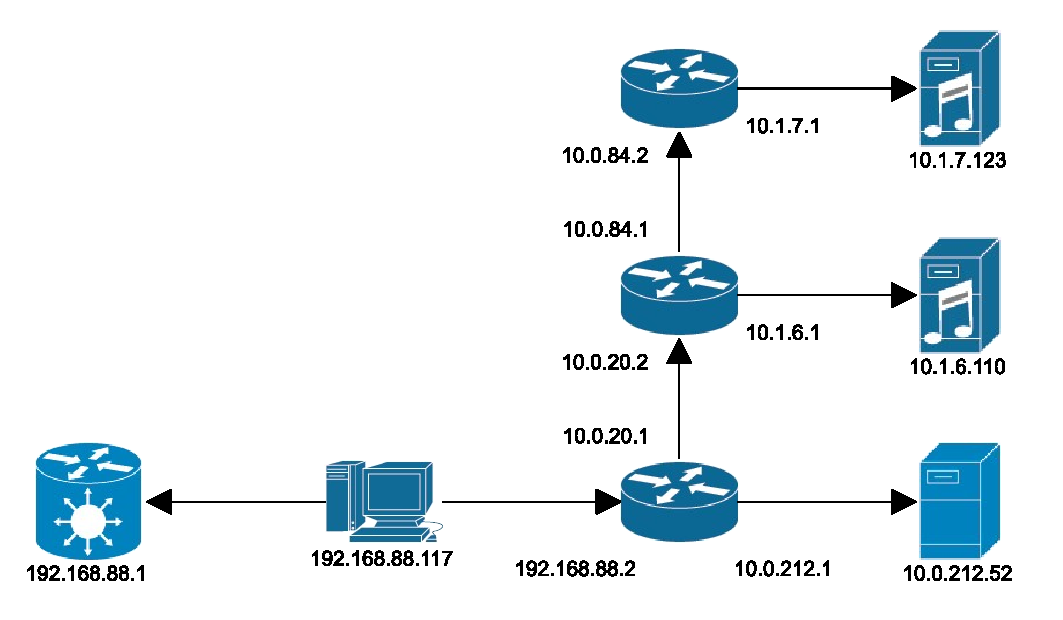
\includegraphics[width=\textwidth]{network_layout.pdf} 
    \caption{Diagram of the network and its different sub-networks}
    \label{fig:networkLayout}
\end{figure}

\subsection{IP of the discovered host}
The IP of the discovered host is \texttt{10.0.212.52}

\subsection{Routing tables of the routers}
The routing tables can be derived from the network diagram (Figure \ref{fig:networkLayout}) and the discovered routes from and to our client (Listing \ref{lst:routes_ping}) are listed in Table \ref{tab:routing}.
Since we don't have enough routing information for \texttt{r2} and \texttt{r3}, we can not discover all routes.

\begin{table}[hb]
    \centering
    \caption{Routing table for our network}
    \label{tab:routing}
    \begin{tabular}{clllc}
        \toprule
        \textbf{router} & \textbf{destination} & \textbf{gateway} & \textbf{interface} & \textbf{hops} \\ \midrule
           & 192.168.88.0/24 & 192.168.88.2 & 192.168.88.2 & 0 \\
           & 10.0.20.0/24    & 10.0.20.2    & 10.0.20.2    & 0 \\
           & 10.0.84.0/24    & 10.0.84.1    & 10.0.84.1    & 0 \\
        r1 & 10.0.212.0/24   & 10.0.212.1   & 10.0.212.1   & 0 \\
           & 10.0.148.0/24   & 10.0.20.1    & 10.0.20.2    & 1 \\
           & 10.1.6.0/24     & 10.0.20.1    & 10.0.20.2    & 1 \\
           & 10.1.7.0/24     & 10.0.20.1    & 10.0.20.2    & 2 \\
        \midrule
           & 10.0.6.0/24     & 10.1.6.1     & 10.1.6.1     & 0 \\
           & 10.0.148.0/24   & 10.0.148.2   & 10.0.148.2   & 0 \\
           & 10.0.20.0/24    & 10.0.20.1    & 10.0.20.1    & 0 \\
        r2 & 10.1.7.0/24     & 10.0.148.1   & 10.0.148.2   & 1 \\
           & 10.0.212.0/24   & 10.0.20.2    & 10.0.20.1    & 1 \\
           & 192.168.88.0/24 & 10.0.20.2    & 10.0.20.1    & 1 \\
           & 10.0.84.0/24    & \textit{unknown} \\
        \midrule
           & 10.1.7.0/24     & 10.1.7.1     & 10.1.7.1     & 0 \\
           & 10.0.84.0/24    & 10.0.84.2    & 10.0.84.2    & 0 \\
           & 10.0.148.0/24   & 10.0.148.1   & 10.0.148.1   & 0 \\
        r3 & 192.168.88.0/24 & 10.0.84.1    & 10.0.84.2    & 1 \\
           & 10.0.212.0/24   & 10.0.84.1    & 10.0.84.2    & 1 \\
           & 10.0.20.0/24    & \textit{unknown} \\
           & 10.1.6.0/24     & \textit{unknown} \\
        \bottomrule
    \end{tabular}
\end{table}

\subsection{Measured network parameters}

The \texttt{ping} and \texttt{mtrace} tools are used to obtain information on the network, especially for the Landline and Satellite hosts.
With \texttt{mtrace}, routers on the way of a packet are discovered by limiting the hop limit of the packet and listening for their expiration message.
Figures \ref{fig:mtraceLandline}, \ref{fig:mtraceSatellite} and Table \ref{tbl:mtraceResults} show the generated results.
We can observe a more severe packet loss on the routers that are between our host and our remote. 
As the packet loss is way lower for packets that shall reach the remote host, we assume that some kind of rate limiting process is taking place in the routers (i.e. router is dropping ICMP packets to save resources).
We observe that Landline experiences no packet loss while Satellite looses 4.2\% of its packets. 
This is the main reason for the degraded QoS that was experienced in Assignment 2.

\begin{table}[hb]
    \centering
    \caption{Results from mtrace}
    \label{tbl:mtraceResults}
    \begin{tabular}{cccccc}
        \toprule
        Destination & Packet Loss [\%] & Avg [ms] & Best [ms] & Worst [ms] & Standard Deviation  \\ \midrule
        Satellite & 4.2 & 961.5 & 939.8 & 2694 & 58.9 \\
        Landline & 0 & 159.1 & 151.6 & 167.1 & 3.2\\
        10.0.20.1 & 27.7 & 159.3 & 151.7 & 166.6 & 3.2\\
        10.0.84.2 & 6.1 & 961.7 & 940.6 & 2794 & 63.0\\
        \bottomrule
    \end{tabular}
\end{table}

\begin{figure}[ht]
    \centering
   \includegraphics[width=\textwidth]{images/mytraceroute1.png} 
    \caption{mtrace to Satellite}
    \label{fig:mtraceSatellite}
\end{figure}

\begin{figure}[ht]
    \centering
   \includegraphics[width=\textwidth]{images/mytraceroute2.png} 
    \caption{mtrace to Landline}
    \label{fig:mtraceLandline}
\end{figure}


\begin{lstlisting}[language=tex, breaklines, frame=single, caption={Landline Network Parameters}, label=lst:landlineNetwork, float, floatplacement=h]
--- 10.1.7.123 ping statistics ---
2023 packets transmitted, 1902 received, 5.98122% packet loss, time 1004ms
rtt min/avg/max/mdev = 939.878/959.329/982.266/11.445 ms, pipe 5
\end{lstlisting}

\begin{lstlisting}[language=tex, breaklines, frame=single, caption={Landline Network Parameters}, label=lst:landlineNetwork, float, floatplacement=h]
--- 10.1.6.110 ping statistics ---
2364 packets transmitted, 2363 received, 0.0423012% packet loss, time 1105ms
rtt min/avg/max/mdev = 151.477/159.317/166.917/3.244 ms
\end{lstlisting}


\subsection{Graphical representation of the measured data (e.g. Histogram, CDF, ...)}

\#TODO: Generate Matlab Graphs that were already used in Assignment 2?
Problem: No Wireshark dumps for this task, only ping data. 
\textit{Use active testing tools to probe the network path between your client and the multimedia services and generate reliable statistics(for links and end-to-end connections) for the QoS-relevant parameters. Display these statistics graphically.}
\subsection{Discussion of the results, comparing with the results from assignment 2}
The measurements of this assignment back up the observations of assignment 2. 
Network performance of the subnets show that the landline sub-network is better (lower packet loss, lower latency) than the satellite sub-network. 

\begin{lstlisting}[language=tex, breaklines, frame=single, caption={Routes discovered by \texttt{traceroute <IP>}}, label=lst:routes_traceroute]
    traceroute 192.168.88.2
     1  border.cn2lab.cn.tuwien.ac.at (192.168.88.2)
    
    traceroute 10.0.20.2
     1  10.0.20.2 (10.0.20.2)
    
    traceroute 10.0.20.1
     1  border.cn2lab.cn.tuwien.ac.at (192.168.88.2)
     2  10.0.20.1 (10.0.20.1)
    
    traceroute 10.0.212.1
     1  10.0.212.1 (10.0.212.1)
    
    traceroute 10.0.212.52
     1  border.cn2lab.cn.tuwien.ac.at (192.168.88.2)
     2  10.0.212.52 (10.0.212.52)
    
    traceroute 10.1.6.1
     1  border.cn2lab.cn.tuwien.ac.at (192.168.88.2)
     2  10.1.6.1 (10.1.6.1)
    
    traceroute 10.1.6.110
     1  border.cn2lab.cn.tuwien.ac.at (192.168.88.2)
     2  10.0.20.1 (10.0.20.1)
     3  landline.cn2lab.cn.tuwien.ac.at (10.1.6.110)
    
    traceroute 10.0.84.1
     1  10.0.84.1 (10.0.84.1)
    
    traceroute 10.0.84.2
     1  border.cn2lab.cn.tuwien.ac.at (192.168.88.2)
     2  10.0.20.1 (10.0.20.1)
     3  10.0.84.2 (10.0.84.2)
    
    traceroute 10.1.7.1
     1  border.cn2lab.cn.tuwien.ac.at (192.168.88.2)
     2  10.0.20.1 (10.0.20.1)
     3  10.1.7.1 (10.1.7.1)
    
    traceroute 10.1.7.123
     1  border.cn2lab.cn.tuwien.ac.at (192.168.88.2)
     2  10.0.20.1 (10.0.20.1)
     3  10.0.84.2 (10.0.84.2)
     4  satellite.cn2lab.cn.tuwien.ac.at (10.1.7.123)
    
    traceroute 192.168.88.1
     1  cn2lab.cn.tuwien.ac.at (192.168.88.1)
    \end{lstlisting}
    
    \begin{lstlisting}[language=tex, breaklines, frame=single, caption={Routes discovered by \texttt{ping -R <IP>}}, label=lst:routes_ping]
        ping -R 192.168.88.2:
            -> 192.168.88.112
            -> 192.168.88.2
            <- 192.168.88.2
            <- 192.168.88.112
    
        ping -R 10.0.212.1:
            -> 192.168.88.112
            -> 10.0.212.1
            <- 10.0.212.1
            <- 192.168.88.112
    
        ping -R 10.0.212.52:
            -> 192.168.88.112
            -> 10.0.212.1
            -> 10.0.212.52
            <- 10.0.212.52
            <- 192.168.88.2
            <- 192.168.88.112
    
        ping -R 10.0.20.2:
            -> 192.168.88.112
            -> 10.0.20.2
            <- 10.0.20.2
            <- 192.168.88.112
    
        ping -R 10.0.20.1:
            -> 192.168.88.112
            -> 10.0.20.2
            -> 10.0.20.1
            <- 10.0.20.1
            <- 192.168.88.2
            <- 192.168.88.112
    
        ping -R 10.1.6.1:
            -> 192.168.88.112
            -> 10.0.20.2
            -> 10.1.6.1
            <- 10.1.6.1
            <- 192.168.88.2
            <- 192.168.88.112
    
        ping -R 10.0.84.2:
            -> 192.168.88.112
            -> 10.0.20.2
            -> 10.0.148.2
            -> 10.0.84.2
            <- 10.0.84.2
            <- 192.168.88.2
            <- 192.168.88.112
    
        ping -R 10.0.84.1:
            -> 192.168.88.112
            -> 10.0.84.1
            <- 10.0.84.1
            <- 192.168.88.112
    
        ping -R 10.1.7.1:
            -> 192.168.88.112
            -> 10.0.20.2
            -> 10.0.148.2
            -> 10.1.7.1
            <- 10.1.7.1
            <- 192.168.88.2
            <- 192.168.88.112
    
        ping -R 10.1.7.123:
            -> 192.168.88.112
            -> 10.0.20.2
            -> 10.0.148.2
            -> 10.1.7.1
            -> 10.1.7.123
            <- 10.1.7.123
            <- 10.0.84.2
            <- 192.168.88.2
            <- 192.168.88.112
    
        ping -R 192.168.88.1:
            -> 192.168.88.112
            -> 192.168.88.1
            <- 192.168.88.1
            <- 192.168.88.112
    \end{lstlisting}

%%%%%%%%%%%%%%%%%%%%%%%%%%%%%%%%%%%%%%%%%%%%%%%
\end{document}
